\documentclass[fontsize=25pt,margin=0.5in,innermargin=-1.8in,blockverticalspace=0.25in]{tikzposter}
\geometry{paperwidth=36in,paperheight=48in}
\usepackage[utf8]{inputenc}
\usepackage{amsmath}
\usepackage{amsfonts}
\usepackage{amsthm}
\usepackage{amssymb}
\usepackage{mathrsfs}
\usepackage{graphicx}
\usepackage{adjustbox}
\usepackage{enumitem}
\usepackage[backend=biber,style=numeric]{biblatex}
\usepackage{SUtheme}
\usepackage{svg}

\graphicspath{ {./img/} }

\usepackage{mwe} % for placeholder images

\addbibresource{refs.bib}

% set theme parameters
\tikzposterlatexaffectionproofoff
\usetheme{SUTheme}
\usecolorstyle{SUStyle}
\usetitlestyle{Filled}

\usepackage[scaled]{helvet}
\renewcommand\familydefault{\sfdefault} 
\usepackage[T1]{fontenc}
\usepackage{adjustbox}
\newtheorem{theorem}{Theorem}
\newtheorem{definition}[theorem]{Problem Definition}

\titlegraphic{\raisebox{0.4\height}{
\includegraphics[width=0.1\textwidth]{UM-logo}}}
\title{Minimizing Interference in 1-dimensional Networks}
\author{\underline{Atishaya Maharjan}, Dr. Stephane Durocher}
\institute{GADA lab, Department of Computer Science, University of Manitoba}

\begin{document}
\maketitle
\centering
\begin{columns}[colspacing=0.1em]
	\column{0.35}
	\block{Background}{
		\textbf{Problem Definition:}
		\begin{definition}
			\textbf{INPUT}:
			\\
			Given a set of wireless nodes represented by a set of points $P \subseteq \mathbb{R}^d$
			\\
			\textbf{OUTPUT}:
			\\
			Assign a \textbf{radius of transmission} to each node in $P$ such that the resulting communication graph is \textbf{connected} and the \textbf{maximum interference is minimized}.
		\end{definition}
		\\
		\textbf{Previous Work:}
		\begin{itemize}
			\item Rickenbach et.al \cite{cite:rickenbach_article} showed that the optimal configuration results in minimum interference $O(\sqrt{n})$ and gave a $\sqrt[4]{n}$ approximation algorithm in 1D.
			\item Buchin \cite{cite:buchin} proved that the MMID is NP-hard in 2 or more dimensions while Von Rickenbach \cite{cite:rickenbach_article}.
		\end{itemize}
	}
	\block{Receiver Centric Model}{
		\begin{itemize}
			\item Rickenbach's receiver-centric wireless network model:
			      \begin{enumerate}
				      \item Nodes are points on a plane with transmission radii $r(p)$.
				      \item Interference at point $p$ is defined as:
				            \[
					            I(p) = |\{q \mid q \in P \setminus \{p\}, p \in D(q, r(q)) \}|
				            \]
				      \item $D(p, r(p))$ represents the transmission circle centered at $p$ with radius $r(p)$.
			      \end{enumerate}
		\end{itemize}
		\vspace{1em}
		\begin{tikzfigure}[Illustration of the interference model]
			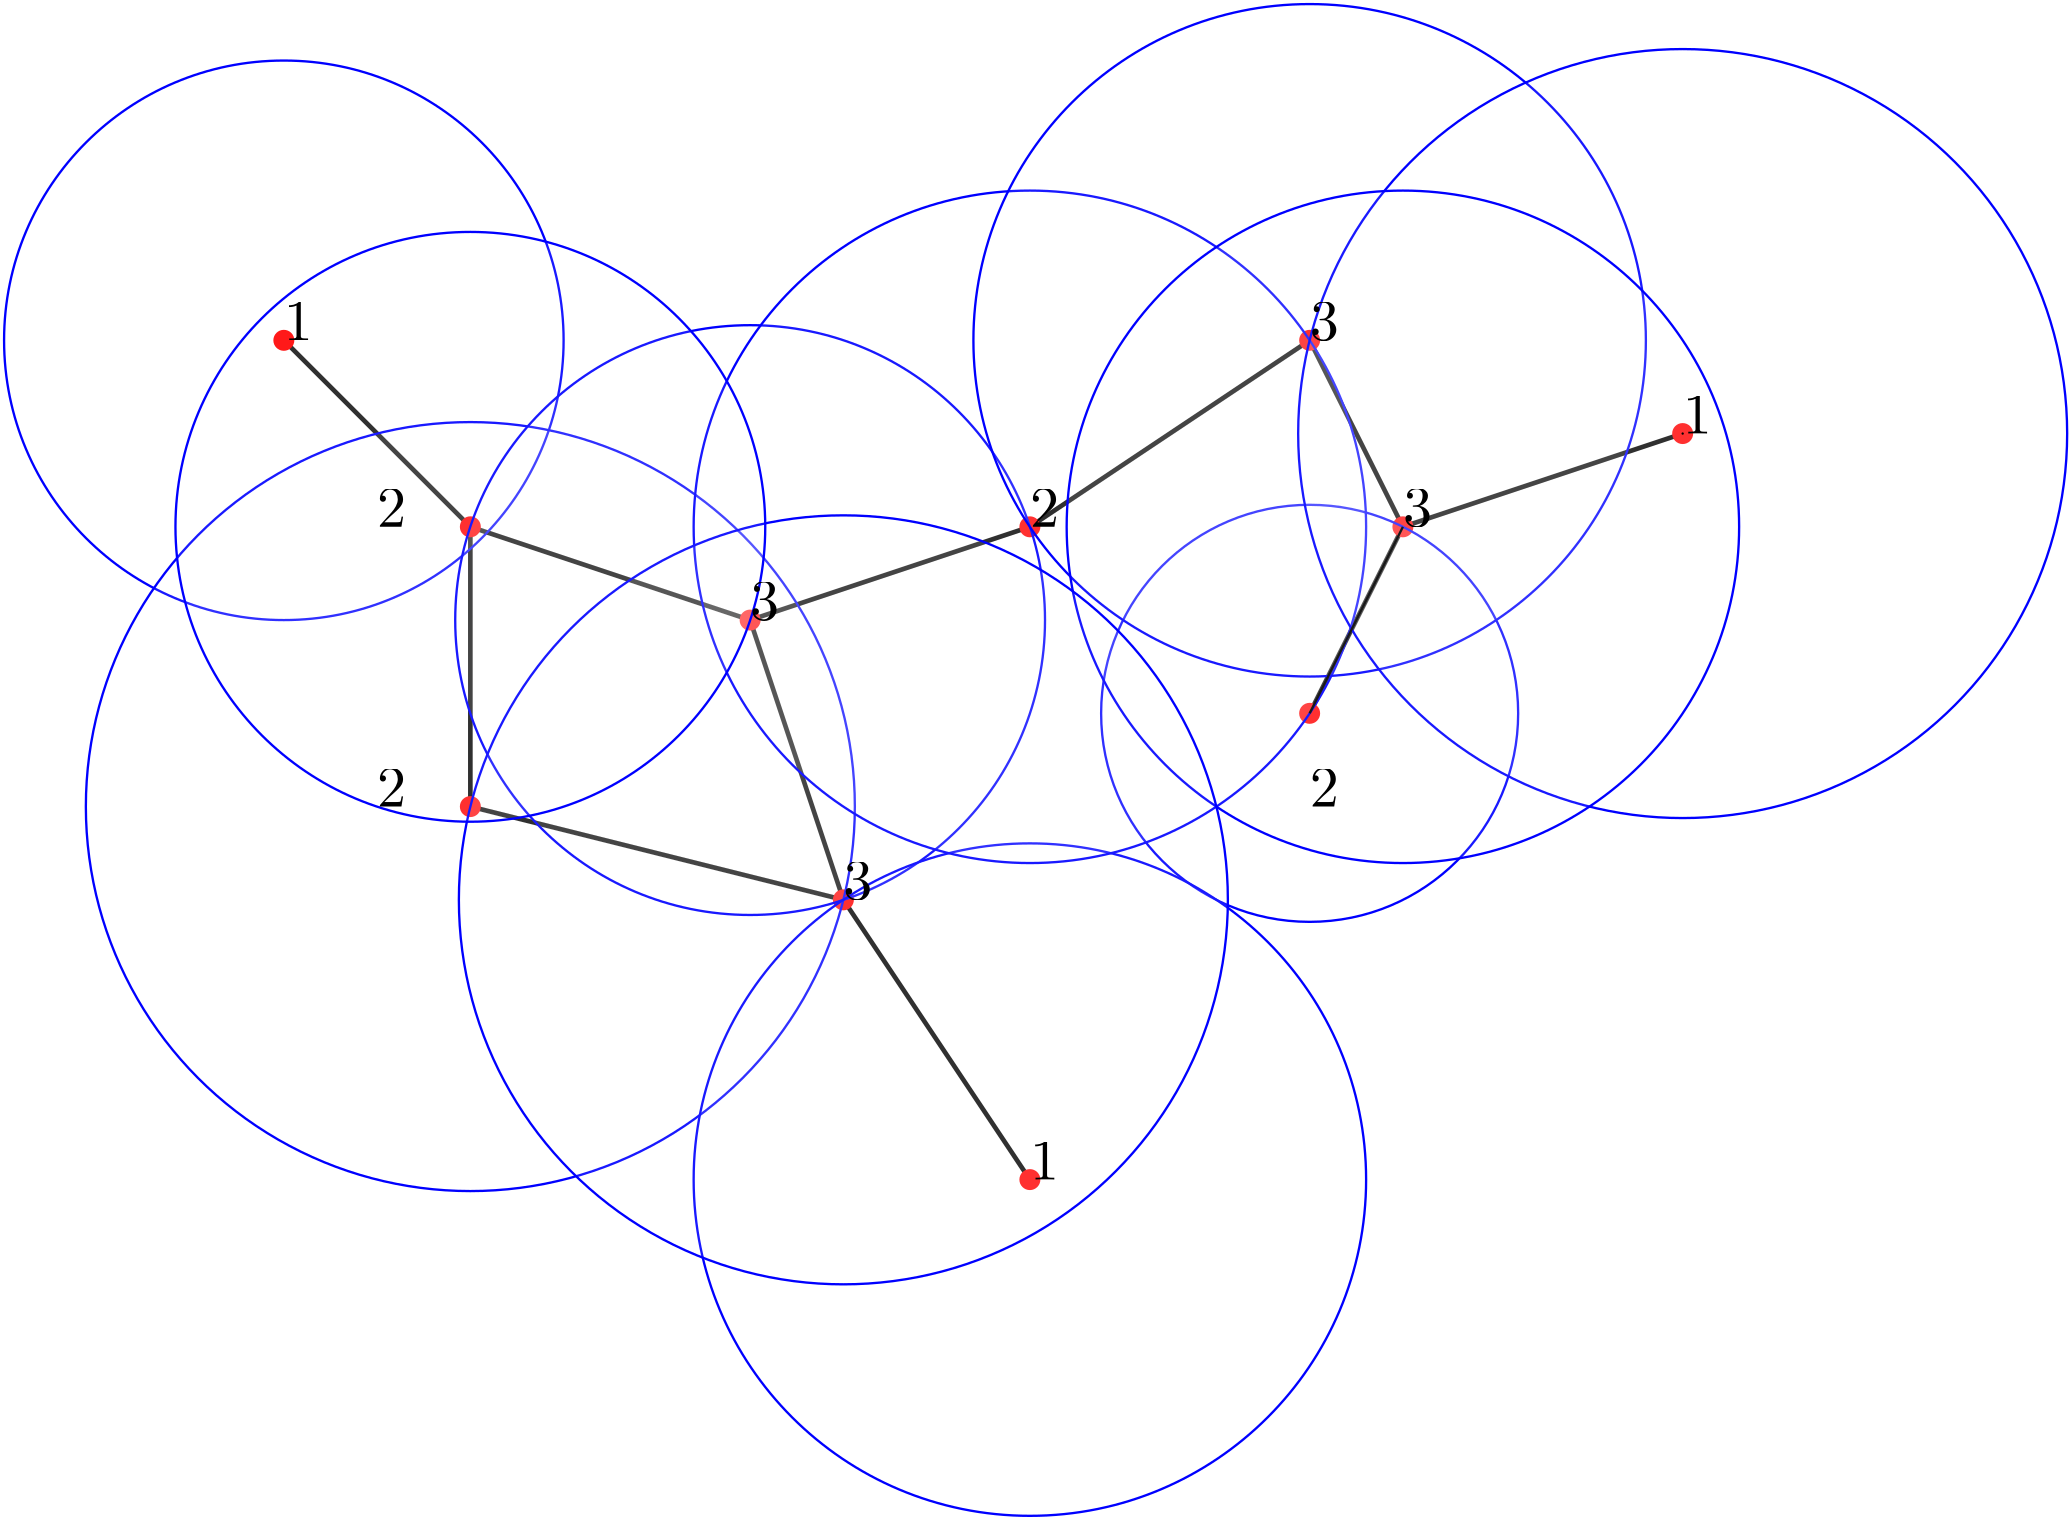
\includegraphics[width=\linewidth]{interference-model}
		\end{tikzfigure}
		\vspace{1em}
	}
	\block{Highway Model} {
		\begin{itemize}
			\item Rickenbach \cite{cite:rickenbach_article} introduced the 1-dimensional model as the highway model:
			      \begin{itemize}
				      \item Points are aligned along a line, similar to vehicles on a highway.
				      \item Worst case: every point interferes with the point on the left.
			      \end{itemize}
		\end{itemize}

		\vspace{1em}
		\begin{tikzfigure}[The starting point has $O(n)$ interference]
			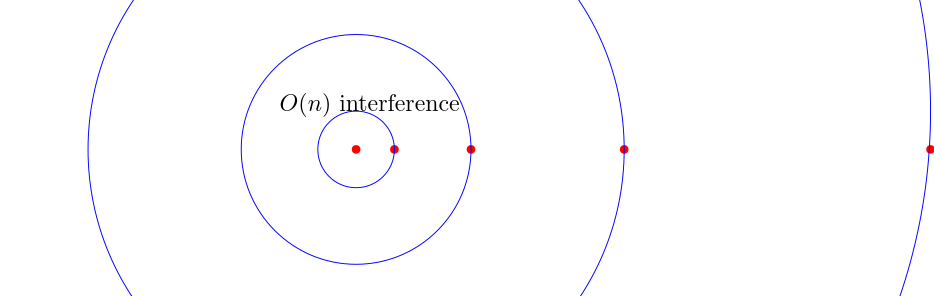
\includegraphics[width=\linewidth]{highway-model-cropped}
		\end{tikzfigure}
		\vspace{1em}


		\vspace{1em}
		\begin{tikzfigure}[The maximum interference is $O(\sqrt{n})$]
			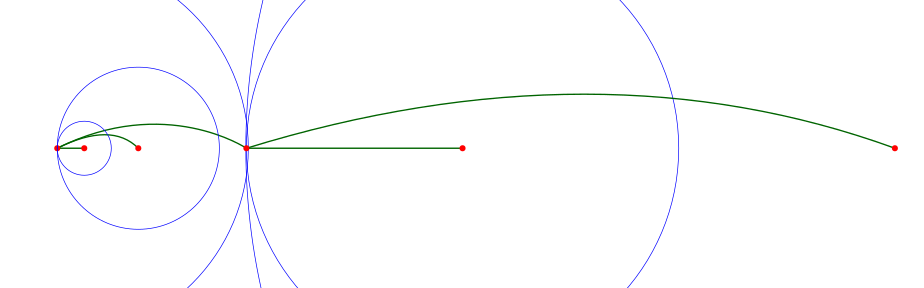
\includegraphics[width=\linewidth]{root-n-interference}
		\end{tikzfigure}
		\vspace{1em}
	}

	\column{0.35}
	\block{Results}{
	The research is still in progress, however here are a few of the ideas illustrated:

	\begin{enumerate}
		\item \textbf{Reduction from $VERTEXCOVER$ to $MTIP$}:
		      \begin{tikzfigure}[Idea 1: A failed reduction from $VERTEXCOVER$ to $MTIP$. The reason why it is not valid is because the reduction presumes the existence of a $k$-vertex cover.]
			      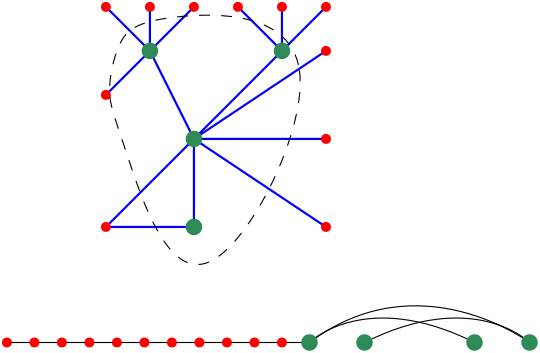
\includegraphics[width=\linewidth]{vertex_cover_reduction}
		      \end{tikzfigure}
		      \vspace{1em}

		\item \textbf{Fixed distance set}:
		      \vspace{1em}
		      \begin{tikzfigure}[Idea 2: Fixed distance set. The distance between the points is fixed and the radius of transmission is optimized. Note that the interference is the ratio of the biggest distance and the smallest distance of the distance set.]
			      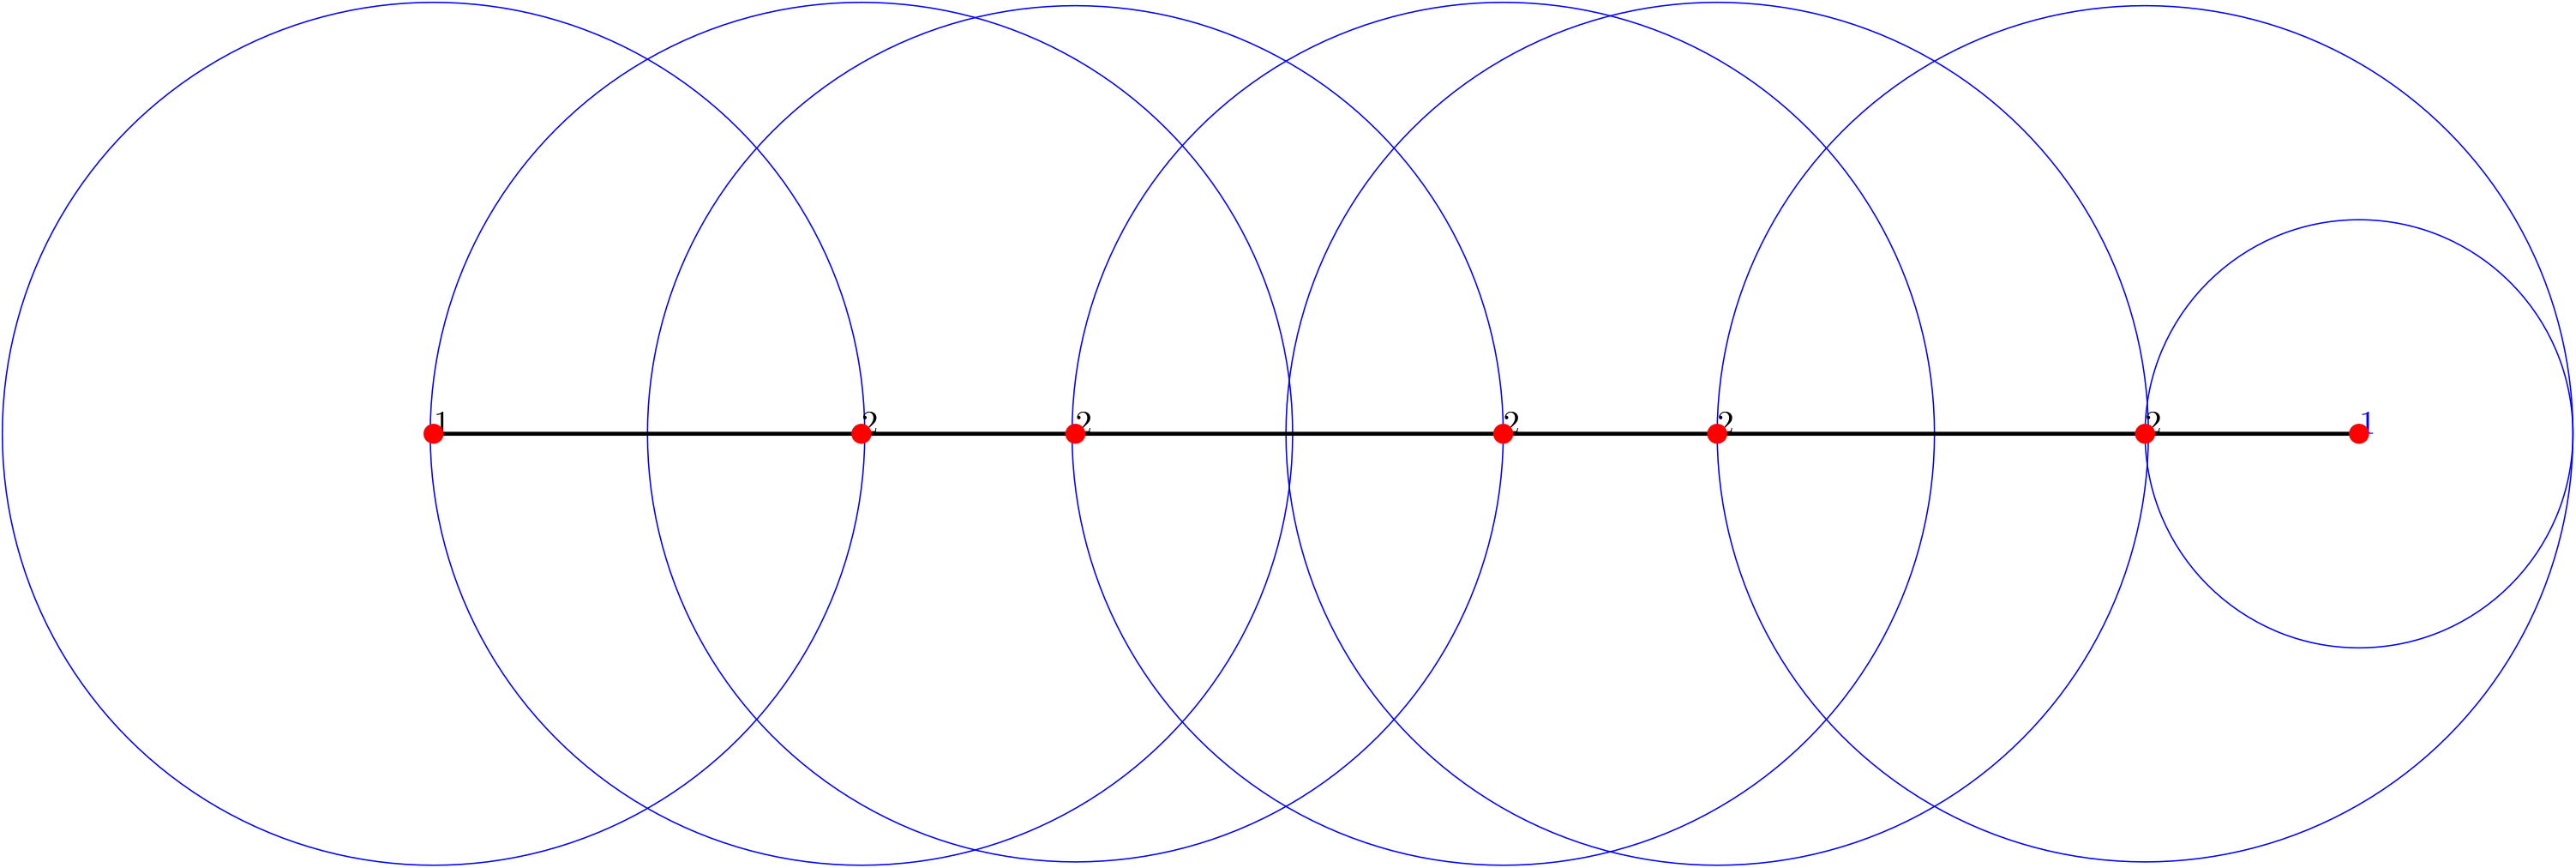
\includegraphics[width=\linewidth]{fixed_distance_set}
		      \end{tikzfigure}
		      \vspace{1em}
	\end{enumerate}

	{\Large\textbf{In progress ideas:}}
	\vspace{1em}

	\begin{enumerate}
		\item \textbf{Adapting the $MTIP$ algorithm for the highway model}: We are trying to adapt the Minimizing Total Interference Problem, $MTIP$, algorithm by Karim \cite{cite:karim} for the highway model.
		      \vspace{1em}
		      \begin{tikzfigure}[Sink tree with 6 nodes, where the uppermost node is the sink node. The maximum interference of this network is 3. The idea of sink trees is vital for ]
			      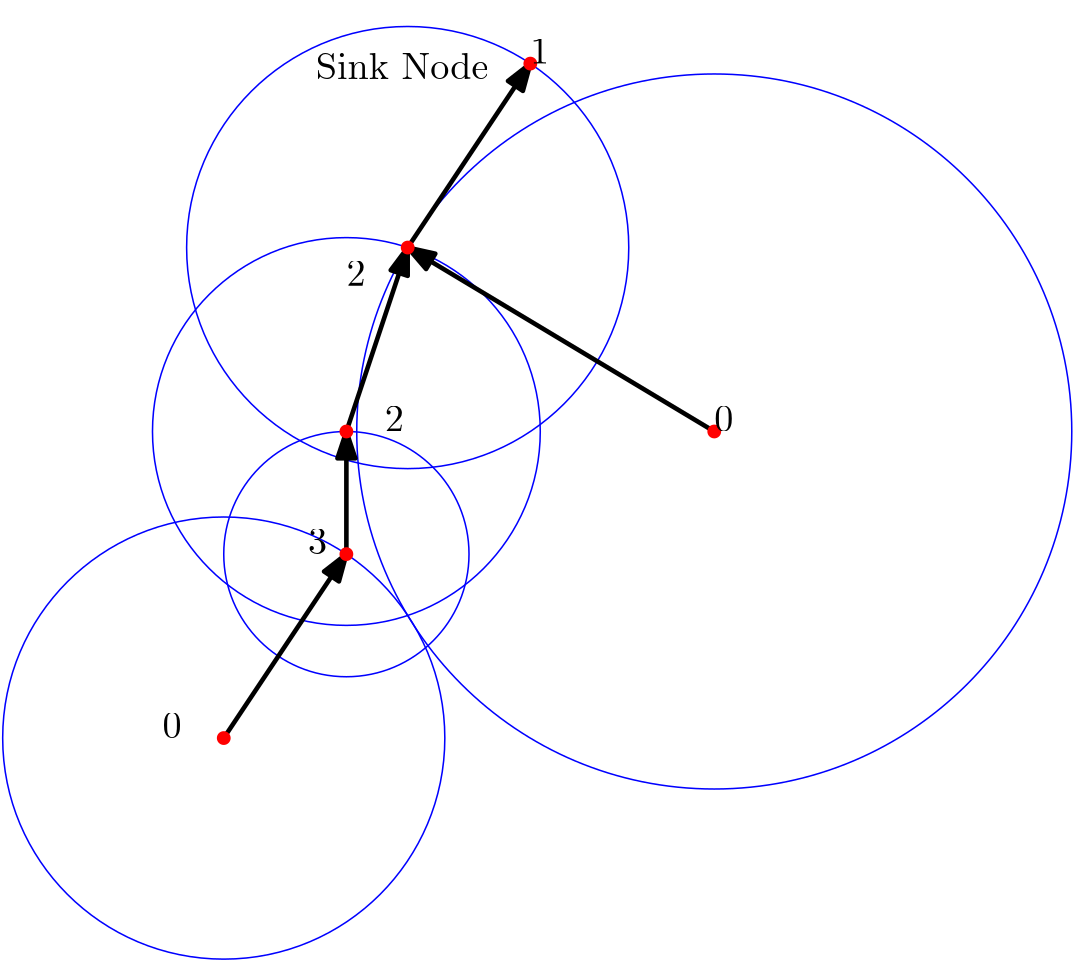
\includegraphics[width=\linewidth]{sink_tree}
		      \end{tikzfigure}
		      \vspace{1em}

		\item \textbf{Fixed Parameter Tractable methods}: Here is the problem definition that we are currently working towards:
		      \vspace{1em}
		      \begin{definition}
			      $ $ \\
			      Given $P = \{p_1, \dots, p_n\} \subseteq \mathbb{R}$ such that $\forall i, p_i < p_{i + 1}$, find an algorithm that finds the optimal solution for $P$ in $O(f(k)\cdot n^c$ time, for some $f(k)$ and $c \in O(1)$.
		      \end{definition}
		      \vspace{1em}
		\item \textbf{Finding a better approximation algorithm than $\sqrt[4]{n}$}: Finding a better $\alpha$ approximation algorithm such that $\alpha < \sqrt[4]{n}$.
	\end{enumerate}
	}

	\column{0.3}
	\block{Comparison}{
		Recent developments in the minimizing interference in networks include looking at minimizing the total interference instead of the maximum interference in a given point set. Karim et. al\cite{cite:karim} showed that you can actually obtain a $O(n^3)$ algorithm that minimizes the total interference. Their definition of interference was as follows:

		\begin{align*}
			I(G_\rho) = \displaystyle\sum_{p \in P}^{RI(p)}
		\end{align*}

		where $RI(p)$ denotes the asymmetric transmission radius of a point $p$.

		Our problem defines the interference as:

		\begin{align*}
			I(G) = \max_{e \in E} Cov(e)
		\end{align*}

		where $Cov(e)$ denotes the coverage of an edge $e$ which is given by:

		\begin{align*}
			Cov(e) = |\{w \in V | w \text{ is covered by } D(u, |uv|)\} \cup \{w \in V | w \text{ is covered by } D(v, |vu|)\}|
		\end{align*}

		\vspace{1em}
		\begin{tikzfigure}[Karim's model of the minimum weight sink tree for asymmetric sensor networks.]
			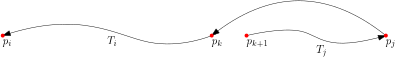
\includegraphics[width=\linewidth]{minimum_weight_sink_tree_asymmetric.png}
		\end{tikzfigure}
		\vspace{1em}

		\vspace{1em}
		\begin{tikzfigure}[Karim's model adapted with symmetric edges which does not reduce the interference level but instead increases it.]
			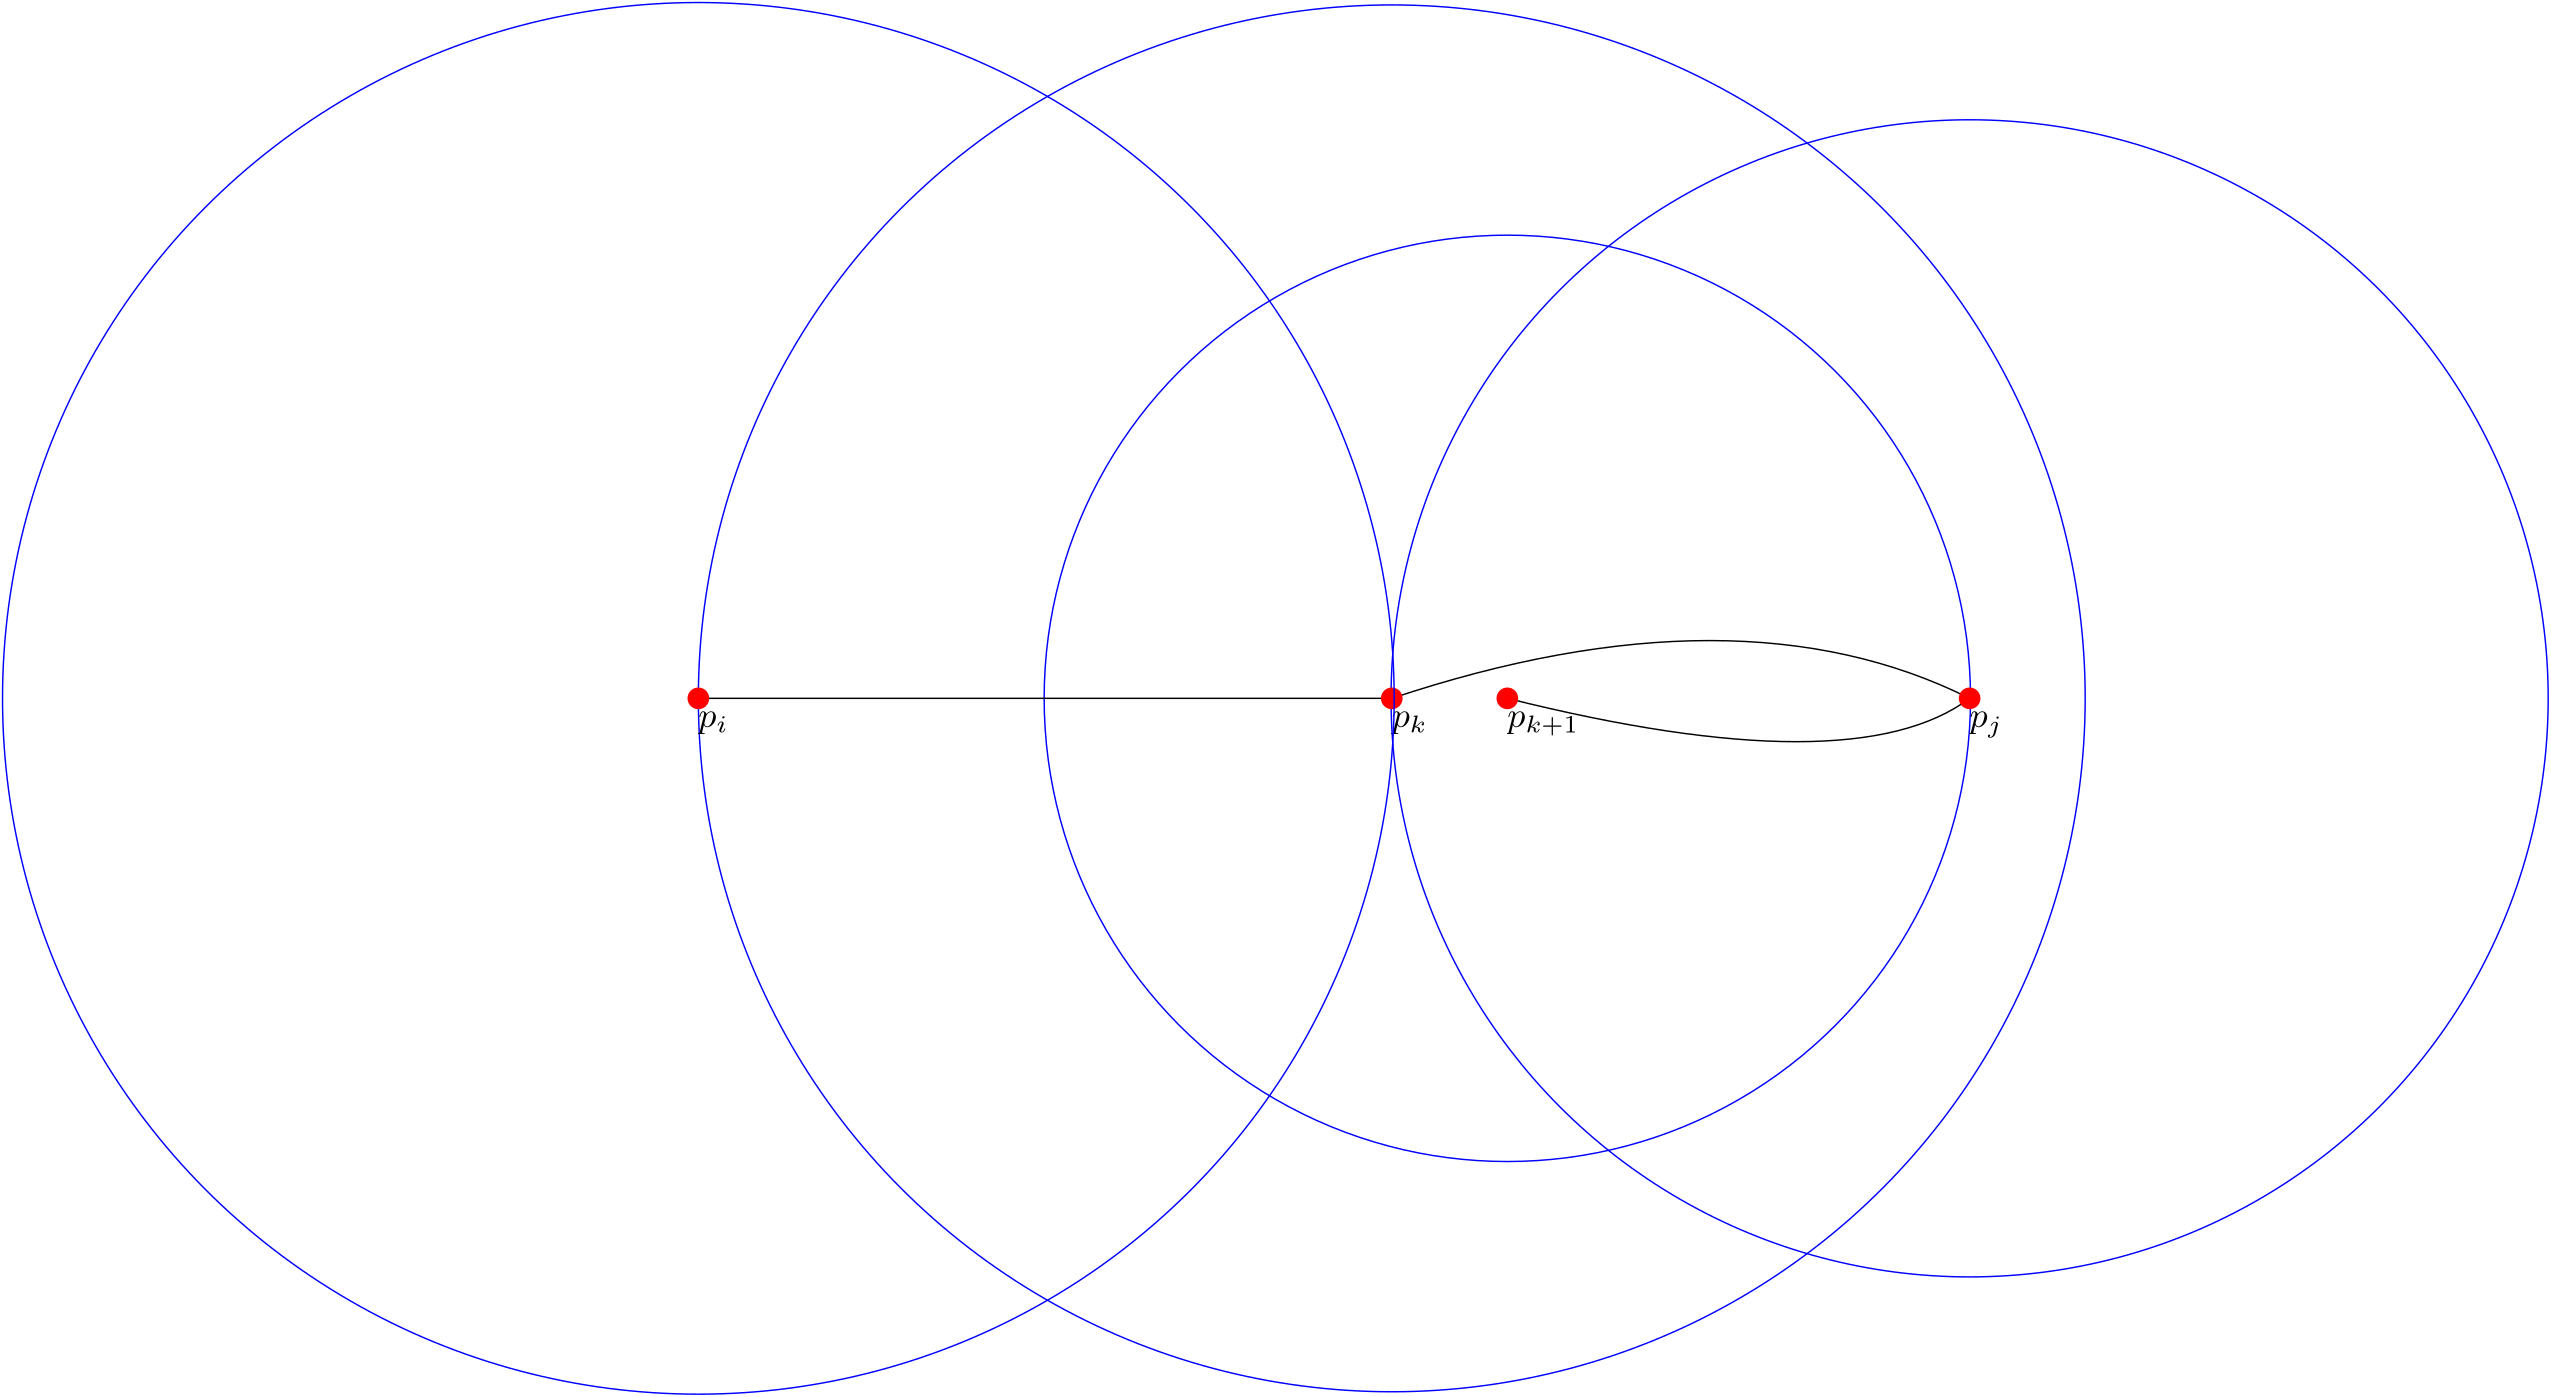
\includegraphics[width=\linewidth]{minimum_weight_sink_tree_symmetric.png}
		\end{tikzfigure}
		\vspace{1em}
	}

	\block{Future Works}{
		\begin{itemize}
			\item Initially believed the problem was NP-hard.
			\item Recent work suggests a high probability of finding a polynomial-time algorithm in possibly other models than the highway model.
			\item Current focus:
			      \begin{itemize}
				      \item Fixed Parameter Tractable methods.
				      \item Adapting the $MTIP$ algorithm for the highway model.
			      \end{itemize}
			\item Successful adaptation may yield a polynomial-time algorithm.
		\end{itemize}
	}

	\block{References}{
		\vspace{-1em}
		\begin{footnotesize}
			\printbibliography[heading=none]
		\end{footnotesize}
	}
\end{columns}
\end{document}
